\chapter{Asimilación de datos en modelos basados en agentes} \label{chp:da_abms}

\section{Modelos basados en agentes}

A diferencia de los modelos de predicción con ecuaciones diferenciales, los modelos basados en agentes (conocidos como ABMs por sus siglas en inglés) se basan en un paradigma diferente. Estos modelan de manera explícita las características y comportamiento de individuos o agentes que interactúan. El comportamiento conjunto de la población de agentes se utiliza como modelo de un sistema complejo \citep{Bonabeau2002}. Incluso reglas de interacción simples pueden resultar en que los agentes se organicen de manera autónoma y que el comportamiento colectivo de la población emerja de manera \textit{bottom-up} desde la escala micro del modelado de los individuos \citep{Helbing2012}. En general, los ABMs requieren una gran capacidad computacional ya que las poblaciones de agentes pueden ser muy grandes. Actualmente es factible utilizarlos de manera operacional y existen ejemplos de su aplicación en epidemiología, ecología, economía y sociología \citep{Vynnycky2010, Grimm2005, Tesfatsion2006, Epstein1996}.

Los modelos de agentes tienen dos componentes principales que los describen: 
\begin{enumerate}
    \item Las descripciones de los agentes mediante atributos
    \item Las reglas de comportamiento e interacción
\end{enumerate}
Los agentes pueden ser vistos como un tipo de dato con diferentes campos de manera que cada individuo se define por el valor de estos atributos. Para completar al modelo se agrega el comportamiento e interacción de los agentes, en general mediante reglas que pueden contener componentes estocásticos. Las acciones que realicen los individuos bajo estas disposiciones provocarán cambios en los valores de sus atributos. En principio estos atributos pueden ser cualquier tipo de dato, de manera que los agentes pueden ser programados como tipos de datos compuestos (como estructuras en C) o incluso a través de clases en lenguajes orientados a objetos. Por ejemplo, se pueden usar números reales para representar coordenadas espaciales, variables categóricas para clases sociales, números enteros para edades, etc.

Para modelar la dispersión de una enfermedad es apropiado construir ABMs epidemiológicos tomando una población de agentes en el que cada uno de ellos representa a una persona o individuo susceptible a contraer y/o transmitir la enfermedad \citep{Roche2011}. Incluso, un agente puede representar a un grupo de individuos de características similares. Utilizando variables categóricas se puede etiquetar a cada agente con su status o categoría epidemiológica (susceptible, infectado, etc.) y estas etiquetas pueden ser cambiadas cuando existe un contacto infeccioso o a medida que la enfermedad se desarrolla en el tiempo. El modelado de los contactos entre agentes admite múltiples representaciones, se pueden hacer mezclas al azar, a través de grupos, con redes de contactos o modelando explícitamente la movilidad de los agentes en el espacio. El uso de ABMs para epidemiología tiene la virtud de que permite modelar de una manera explícita, y con gran detalle, características relevantes del sistema que suceden en la micro-escala de la interacción entre individuos. Por ejemplo, la disminución de la inmunidad puede ser representada en cada individuo a través de un atributo. Es posible modelar de manera natural medidas de control como cuarentenas, rastreo de contactos o efectos de vacunación \citep{Silva2020}. Muchos modelos de ecuaciones diferenciales asumen que dentro de cada compartimento la mezcla entre individuos es homogénea; para ABMs epidemiológicos, al disponer de caracterizaciones de cada individuo, es posible obtener patrones de interacción mas ricos a través de redes de contacto o el mecanismo que resulte más conveniente. De esta manera se pueden capturar efectos difíciles de representar con modelos de ecuaciones diferenciales. A pesar de disponer de información de cada agente, en la simulación con ABMs el interés está en el comportamiento global del sistema. Se suele contar con una función que de alguna manera resuma al estado de la población como un todo a través de un conjunto de variables que llamaremos variables agregadas. En general, si tenemos que la población de agentes es $A$, llamaremos $\v x$ a las variables agregadas y $\phi$ a la función sintetizante o agregante que realiza el mapeo, de manera que:
\begin{align}
    \phi (A) = \v x
\end{align}
El comportamiento de las variables agregadas emergerá del comportamiento a nivel individual del ABM. En el caso de modelos epidemiológicos es razonable, por ejemplo, utilizar como resumen el conteo de la cantidad de individuos en cada categoría para saber cuantos susceptibles, infectados, recuperados, etc. hay.

Con el surgimiento de la pandemia de COVID-19 se han desarrollado una gran diversidad de ABMs. Algunos de estos incorporan, entre otras características, estructura de edades y redes de contactos a través de escuelas, casas, lugares de trabajo que permiten modelar de manera más realista las mezclas que dan lugar a los contactos \citep{Kerr2020,Flaxman2020,Simoy2021}. Además de que el aumento de la capacidad de cómputo hace más viable la utilización de ABMs, el gran caudal de datos recolectados a nivel individual a través de dispositivos electrónicos es otro gran aliciente para el incremento en su popularidad. En \cite{Aleta2020} se utilizan datos demográficos y de movilidad para construir las redes de contactos y distribución de hogares en un ABM que permite evaluar los efectos de las intervenciones no-farmacéuticas.

A pesar de la flexibilidad y expresividad que permite el modelado mediante agentes, sigue siendo necesario calibrarlos adecuadamente. En general, el aumento en complejidad viene acompañado de un aumento en el número de parámetros, los cuales no siempre son especificables a través del conocimiento que se tenga sobre el sistema. Ha habido avances en el desarrollo de técnicas de inferencia para estimar parámetros en ABMs utilizando observaciones. Estos están principalmente orientados a la maximización de la verosimilitud. En particular en \cite{Hooten2020} se discuten una variedad de métodos para maximizar aproximaciones de la verosimilitud usando cómputo Bayesiano aproximado (o ABM por \textit{Approximate Bayesian Computation}) junto con técnicas de MCMC (\textit{Markov Chain Monte Carlo}).

Como los ABMs se enmarcan en un contexto de sistemas con evolución temporal parcialmente observados, es posible pensar que la caja de herramientas provista por la asimilación de datos secuencial es potencialmente de utilidad para realizar las tareas de inferencia. Un trabajo pionero en esta dirección es \cite{Ward2016} en el que se utiliza el EnKF para asimilar datos de cámaras en calles de Leeds con un modelo de agentes para estudiar el comportamiento del tráfico peatonal. A pesar de obtener resultados satisfactorios, se señala la dificultad asociada a la sensibilidad respecto a parámetros del modelo y la necesidad optimizar el código para modelos de gran tamaño. Como mencionamos anteriormente, el interés no necesariamente está puesto en el estado de cada individuo sino en el estado global del sistema o de un conjunto de variables que den una descripción de la población de agentes que se considere relevante. Además, a pesar de que el estado a la escala microscópica determina de manera total al sistema y que el objetivo de la inferencia fuera, idealmente, representar esta escala de la manera más precisa posible, sucede que usualmente las observaciones que se tienen del sistema son de las variables sintetizantes, es decir de la escala macroscópica. Esto significa que las observaciones pueden no tener suficiente ``resolución'' como para que se pueda determinar el estado de los atributos de cada agente. Nuestra propuesta, publicada en \cite{Cocucci2022}, es la de asimilar datos sobre las variables agregadas mediante técnicas basadas en ensambles. El mapeo de la escala microscópica a macroscópica está dado por la función sintetizante $\phi$ pero no tenemos una representación para su inversa. De hecho $\phi$ puede no ser inyectiva y por lo tanto no-invertible: muchas configuraciones de los agentes pueden resultar en el mismo estado de las variables agregadas. Esta situación debe considerarse, a la hora de asimilar observaciones, para hacer un emparejamiento entre los estados macroscópicos observados y el estado de los atributos de los individuos. En este capítulo presentamos un esquema general de aplicación de métodos de asimilación de datos por ensambles para ABMs y dos implementaciones particulares para un ABM epidemiológico que especificamos a continuación.

\section{Modelo epiABM} \label{sec:epi_abm}

Aquí especificamos un ABM epidemiológico diseñado para modelar la dinámica de contagio de enfermedades infecciosas, en particular para el COVID-19 y que denominaremos epiABM. Este es un modelo sencillo para evaluar el rendimiento de la metodología para aplicar asimilación de datos por ensambles en ABMs. Si se quisieran realizar predicciones o asesorar en toma de decisiones, este debería ser adaptado para ese propósito incorporando otras características (por ejemplo, el surgimiento de nuevas cepas y mayor complejidad en la movilidad de agentes).

En el modelo epiABM, el estado de salud de cada agente está descripto por una etiqueta para representar una entre siete categorías. Tenemos a los susceptibles a contraer la enfermedad ($S$). También consideramos a los expuestos a la enfermedad pero que aún no son infecciosos debido a que el virus está incubando ($E$). Después de estar expuestos pasan a una de dos posibles clases de infecciosos. Los infectados leves ($I_M$) son los que desarrollan una sintomatología que no requiere hospitalización y que eventualmente se recuperan. Los infectados graves ($I_S$) son los que requerirán hospitalización. Por su parte, los hospitalizados pueden recuperarse o morir. La categoría $R$ denomina a los recuperados y la $D$ a los muertos. Asumimos que los recuperados adquieren inmunidad permanente, lo cual no es una suposición realista para simulaciones a largo plazo de COVID-19 puesto que las reinfecciones son posibles. El diagrama de la Figura \ref{dia:epi_abm} representa de manera esquemática la progresión de la enfermedad a través de estos estadios.

\begin{figure}
    \begin{center}
        \tikzstyle{block} = [rectangle, draw, fill=blue!20, 
        text width=4em, text centered, rounded corners, minimum height=3em]
        \tikzset{line/.style={draw, very thick, color=black!100, -latex'}}
        \centering
        \begin{tikzpicture}[node distance = 2cm, auto]
            \tikzstyle{block} = [rectangle, draw, fill=blue!20, 
            text width=2em, text centered, rounded corners, minimum height=3em]
            
            % Place nodes
            \node [block] (S) {$S$};
            \node [block, right of=S] (E) {$E$};
            \node [block, above right = 0.05cm and 1cm of E] (IM) {$I_M$};
            \node [block, below right = 0.05cm and 1cm of E] (IS) {$I_S$};
            \node [block, right of=IS] (H) {$H$};
            \node [block, right of=H] (D) {$D$};
            \node [block] (R) at (IM-|D) {$R$};
            
            % Draw edges
            \draw[line] (S) -- (E);
            \draw[line] (E) |- node [below] {$q_S$} (IS);
            \draw[line] (E) |- node [above] {$1-q_S$} (IM);
            \draw[line] (IM) -- (R);
            \draw[line] (IS) -- (H);
            \draw[line] (H) -- node [above] {$q_D$} (D);
            \draw[line] (H) -- node [left = 0.01cm] {$1-q_D$} (R);
        \end{tikzpicture}
    \end{center}
    \caption{Diagrama de las categorías epidemiológicas del modelo epiABM.}
    \label{dia:epi_abm}
\end{figure}

En cada paso temporal, que consideraremos de un día, cada agente tendrá un número de contactos muestreado de una distribución Poisson de parámetro $\lambda$. Los agentes susceptibles podrán resultar infectados por un contacto con un agente infeccioso. El tiempo de permanencia de un agente en las categorías ``intermedias'' ($E$, $I_M$, $I_S$, $H$) está muestreado de una distribución Gamma. Si nombramos a este tiempo $\tau_c$ con $c \in \{E, I_S, I_M, H\}$ entonces $\tau_c \sim \Gamma(k_c, \theta_c)$ donde $k_c$ y $\theta_c$ son los parámetros de forma y escala respectivamente. Con esta parametrización, la media $\mu_c$ y la varianza $\sigma^2_c$ cumplen con las relaciones $\mu_c = k_c \theta_c$ y $\sigma^2_c = k_c \theta_c^2$. El tiempo $\tau_c$ es muestreado para cada agente cuando este entra a la categoría $c$ y cuando este tiempo expira, el agente pasa a la siguiente categoría. Cuando un agente sale de la categoría $E$, tiene una probabilidad $q_S$ de tener una enfermedad severa y $q_M = 1 - q_S$ de que su enfermedad sea leve. Análogamente, los hospitalizados tienen una probabilidad $q_D$ de morir y $q_R = 1 - q_D$ de recuperarse.

Además de la estructura dada por el estatus epidemiológico, incluimos información demográfica y geográfica. El modelo considera una ciudad dividida en $N_{loc}$ comunas. Cada agente vive en una casa (solo o con otros agentes) en una determinada comuna. El tamaño de los hogares sigue una distribución determinada por el vector de probabilidades $p_H$ en el cual la $i$-ésima entrada determina la probabilidad de que un hogar tenga $i$ miembros. Los contactos entre agentes pueden entonces ser definidos en base a esta estructura sencilla. Diferenciaremos entre contactos domésticos y casuales. Cada uno de los contactos diarios de los agentes tiene una probabilidad $q_C$ de ser casual y $1 - q_C$ de ser doméstico. Los contactos domésticos se dan solamente entre miembros de un mismo hogar mientras que los casuales pueden ser, potencialmente con cualquier otro agente. Llamamos $\beta_D$ (respectivamente $\beta_C$) a la probabilidad de que un contacto doméstico (respectivamente casual) sea infeccioso. De esta manera podemos escribir una expresión para el valor esperado de la probabilidad de infección global como $\beta = q_C \beta_C + (1 - q_C) \beta_D$. Por su parte, los contactos casuales van a estar mediados por la conectividad entre los diferentes barrios. Llamaremos $C_{ij}$ a la probabilidad de que un contacto casual de un agente del barrio $j$ se de con un agente del barrio $i$. Esto resulta en una matriz $C$ de tamaño $N_{loc} \times N_{loc}$ que nombraremos matriz de contacto. Los elementos de la diagonal corresponden a la probabilidad de que un contacto casual se de entre habitantes del mismo barrio mientras que los elementos fuera de ella tienen que ver con los contactos entre habitantes de barrios distintos. La matriz $C$ codifica entonces la movilidad entre barrios que a su vez se relaciona a las actividades sociales y laborales de la ciudad. El diseño de esta matriz puede incluir diferentes características de la estructura social y geográfica de la ciudad. Por ejemplo, sería esperable que los agentes transiten con más frecuencia su propio barrio, lo que implicaría valores más altos en los elementos de la diagonal y más pequeños por fuera de esta. Por otro lado, en caso de tener un barrio con más tránsito, por ejemplo un barrio céntrico, los valores correspondientes por fuera de la diagonal serían mayores que en el caso de un barrio menos visitado. Para este trabajo consideraremos que $C$ está fija en el tiempo pero existe la posibilidad de diseñar esta matriz con mayor detalle: por ejemplo se podría ajustar utilizando datos de movilidad que varíen en el tiempo para contemplar cambios que afecten al contacto entre personas o incluso para incluir los efectos de medidas de control como cuarentenas o restricciones de movilidad. Aquí utilizamos expresiones sencillas para la matriz de contactos porque el objetivo principal es el de la evaluación de la metodología propuesta para asimilar datos en ABMs. Una parametrización por defecto para el modelo se especifica en el Apéndice \ref{appendix:epi_abm_default_params}.

El modelo puede ser extendido añadiendo más atributos a los agentes o representando con mayor detalle los patrones de contacto entre personas. Por ejemplo, sería posible incorporar edades o perfiles sociales para enriquecer la configuración de relaciones entre contactos que sean relevantes para la descripción de la dispersión de la enfermedad. Añadir eventos sociales de gran concurrencia, como por ejemplo lugares de trabajo o escuelas puede ser útil para el modelado de los fenómenos de dispersión masiva (conocidos como eventos \textit{superspreader}). También es posible incluir otras características como las campañas de vacunación o el surgimiento de nuevas cepas del virus. Incorporando campos a la descripción del estado de los agentes se puede determinar si están vacunados, cuantas dosis recibieron, etc. Por otro lado, se podría indicar con qué variante del virus se contagiaron los agentes infectados.

El ABM subdivide al total de agentes en subpoblaciones de acuerdo a categorías epidemiológicas de manera similar a modelos compartimentales de ecuaciones diferenciales. Sin embargo los ABMs no pueden ser descriptos de manera directa con ecuaciones diferenciales. Cuando el número de agentes es grande las variables agregadas pueden suavizar el efecto de las componentes estocásticas (por ejemplo de los tiempos muestreados de distribuciones Gamma) y como resultado pueden llegar a ser reproducibles con modelos de ecuaciones diferenciales. Los ABMs tienen características, tal como el comportamiento resultante de tener agentes que residen en hogares y con tasas de infección diferenciadas entre contactos domésticos y casuales, para las cuales no está claro cómo se podrían traducir a un modelo basado en ecuaciones. El modelado a nivel microscópico de los ABMs puede tener consecuencias en la gran escala que pueden no ser fáciles de predecir. A pesar de esto, es importante destacar que los ABMs pueden tener un alto costo computacional lo cual ha motivado el uso de modelos de ecuaciones que actúan como sustitutos de un ABM y que pueden ser utilizados para realizar inferencia con bajo costo computacional \citep{Hooten2020}.

\section{Asimilación de datos en ABMs}

Para aplicar técnicas de asimilación de datos a ABMs es necesario entender primero que el estado propiamente dicho de un sistema de agentes en un instante de tiempo $t$ está dado por el valor de los atributos de cada uno de los agentes que componen la población. En principio no es conveniente aplicar asimilación de datos en un espacio de estas características porque, por un lado, la cantidad de variables es enorme (del orden de la cantidad de agentes multiplicado por la cantidad de atributos) y por otro lado muchos de los atributos pueden no ser valores numéricos. Es posible aplicar filtros de partículas sobre espacios con variables categóricas pero apuntamos a usar el EnKF el cual trabaja sobre espacios de números reales. Incluso de ser factible asimilar datos en el espacio dado por los atributos de los agentes es probable que el interés principal esté en la inferencia sobre las variables agregadas. En el caso del modelo epiABM las variables agregadas estarán dadas por la cantidad de agentes con determinados atributos (por ejemplo estado epidemiológico y comuna). Estos valores son enteros pero al ser lo suficientemente grandes pueden ser tratados por el EnKF como si pertenecieran a un espacio continuo. Además de este punto notemos que, en general las observaciones sobre el sistema serán sobre las variables agregadas, por lo que serán más informativas sobre el valor de estas cantidades y por lo tanto es más directo intentar la inferencia sobre el espacio que estas determinan.

Llamaremos al conjunto de valores de atributos del $k$-ésimo agente en una población a tiempo $t$ como $A_{k, t}$. A su vez, al conjunto de estos valores para toda la población de agentes la llamaremos $A_t = \{ A_{k, t} \}_{k=1}^{N_a}$, donde $N_a$ es el número total de individuos. Debido a que nuestro enfoque apunta a utilizar técnicas basadas en muestras debemos considerar que tenemos no una población sino un ensamble de tamaño $N_p$ de poblaciones de tamaño $N_a$. Este ensamble puede ser representado como $\{ A_{t}^{(j)} \}_{j=1}^{N_p}$. Por su parte, el proceso de asimilación de datos se dará sobre las variables agregadas, o macroscópicas, $\v x_t$. Estas se pueden obtener de una población de agentes $A_t$ mediante la aplicación de la función sintentizante, de manera que tenemos $\v x_t = \phi (A_t)$. De esta manera tenemos el ABM para evolucionar temporalmente a la población de agentes de $A_t$ a $A_{t+1}$ y mediante $\phi$ podemos obtener las variables agregadas $\v x_{t+1}$. El inconveniente es que la función $\phi$ no será en general inyectiva y por lo tanto no será invertible, es decir que muchas configuraciones distintas de la población de agentes pueden dar las mismas variables agregadas. La técnica de asimilación de datos actualiza las variables sobre las que actúa cuando incorpora la información de una observación. En nuestro caso se actualizará a $\v x$ pero como $\phi$ no es invertible no tenemos una manera explícita de dar cuenta de este cambio sobre la población de agentes. Es importante notar que tanto para el EnKF como para el filtro de partículas el modelo es tratado como una caja negra por lo que estas técnicas actuarán ignorando por completo la existencia del mapeo $\phi$.

Al tiempo $t$ supongamos que tenemos un ensamble $\{ A_{t}^{f(j)} \}_{j=1}^{N_p}$. Cada miembro del ensamble $A_{t}^{f(j)}$ representa una población de agentes donde el supraíndice $f$ indica que la muestra es de un \textit{forecast}. Para obtener un pronóstico de las variables de estado simplemente debemos aplicar $\phi$ a cada $A_{t}^{f(j)}$ y de esa manera conseguimos el ensamble $\{ \v x_{t}^{f(j)} \}_{j=1}^{N_p}$. Utilizando este pronóstico en combinación con la observación $\v y_t$ obtenemos, mediante la actualización de la técnica de asimilación de datos, un ensamble de análisis $\{ \v x_{t}^{a(j)} \}_{j=1}^{N_p}$. En este punto, en un esquema de asimilación de datos por ensambles tradicional utilizaríamos el modelo para evolucionar $\{ \v x_{t}^{a(j)} \}_{j=1}^{N_p}$ en $\{ \v x_{t+1}^{f(j)} \}_{j=1}^{N_p}$, es decir que con las variables de estado de análisis a tiempo $t$ obtendríamos un pronóstico a tiempo $t+1$. Pero el ABM no puede transformar directamente $\v x_t$ en $\v x_{t+1}$ sino que evoluciona a $A_t$ en $A_{t+1}$. Necesitamos entonces una representación de agentes $A_{t}^{a(j)}$ de las variables $\v x_{t}^{a(j)}$. Esta población de agentes puede entonces ser usada por el ABM para obtener las poblaciones de agentes de pronóstico $\{ A_{t+1}^{f(j)} \}_{j=1}^{N_p}$ para el tiempo siguiente y retomar la iteración pronóstico-análisis. En la Figura \ref{dia:ensemble_DA_ABM} se sintetiza este procedimiento general. El ingrediente faltante entonces es el ajuste de la población de agentes a las variables agregadas actualizadas mediante la información observacional. Para esto proponemos dos metodologías distintas para el caso del epiABM.

\begin{figure}
\captionsetup{width=0.5\textwidth}
\begin{center}
\tikzset{line/.style={draw, very thick, color=black!100, -latex'}}
\begin{tikzpicture}[node distance = 3cm, auto]
    \tikzstyle{block} = [rectangle, draw, fill=blue!20, 
    text width=5em, text centered, rounded corners, minimum height=3em]
    \tikzstyle{observation} = [circle, draw, fill=blue!20, 
    text width=1.5em, text centered, rounded corners, minimum height=1em]

    % Place nodes
    \node [block] (Af) {$\{A_t^f\}_{j=1}^{N_p}$};
    \node [block, below = 1cm of Af] (xf) {$\{ \v x_t^f\}_{j=1}^{N_p}$};
    \node [observation, below right=0.5cm and -0.5cm of xf] (y) {$\v y_t$};
    \node [block, below of=xf] (xa) {$\{ \v x_t^a\}_{j=1}^{N_p}$};
    \node [block, below = 1cm of xa] (Aa) {$\{A_t^a\}_{j=1}^{N_p}$};

    \node [block, right=2cm of Af] (Af1) {$\{A_{t+1}^f\}_{j=1}^{N_p}$};
    \node [block, below = 1cm of Af1] (xf1) {$\{ \v x_{t+1}^f\}_{j=1}^{N_p}$};
    \node [observation, below left=0.5cm and -0.5cm of xf1] (y1) {$\v y_{t+1}$};
    \node [block, below of=xf1] (xa1) {$\{ \v x_{t+1}^a\}_{j=1}^{N_p}$};
    \node [block, below = 1cm of xa1] (Aa1) {$\{A_{t+1}^a\}_{j=1}^{N_p}$};

    \coordinate[below left = 1cm and 1cm of Aa] (aux);
    \coordinate[below right = 1cm and 1cm of Aa1] (aux1);
    \coordinate[left = 0.5cm of Af] (prev);
    \coordinate[right = 0.5cm of Aa1] (follow);

    % Draw edges
    \draw[line] (Af) -- node [left] {$\phi$}  (xf);
    \draw[line] (xf) -- node [left, text width=2cm, align=right] {Asimilación}  (xa);
    \draw[line] (xa) -- node [left, text width=3cm, align=right] {Ajuste de\\ agentes}  (Aa);
    \draw[line] (y) -- ($(xa.north) + (0.25cm, 0cm)$);

    \draw[line] (Aa.north east) -- node [sloped, below, midway] {ABM} (Af1.south west);

    \draw[line] (Af1) -- node [right] {$\phi$} (xf1);
    \draw[line] (xf1) -- node [right, text width=2cm, align=left] {Asimilación} (xa1);
    \draw[line] (xa1) -- node [right, text width=3cm, align=left] {Ajuste de\\ agentes} (Aa1);
    \draw[line] (y1) -- ($(xa1.north) - (0.25cm, 0cm)$);

    \draw[line] (aux) -- node {Tiempo} (aux1);
    \path (prev) -- node[auto=false]{\ldots} (Af);
    \path (Aa1) -- node[auto=false]{\ldots} (follow);

\end{tikzpicture}
\caption{Esquema general de asimilación de datos por ensambles para ABMs}
\label{dia:ensemble_DA_ABM}
\end{center}
\end{figure}

\subsection{Metodologías de ajuste de agentes} \label{sec:agents_adjustment}

Para aplicar el esquema propuesto es necesario entonces construir una población de agentes consistente con el estado de las variables macro una vez que estas fueron actualizadas por el sistema de asimilación de datos. El problema es que para cada $j = 1, ..., N_p$ tendremos una discordancia entre las variables de estado de la población de agentes que tenemos como pronóstico $\v x_t^{f(j)} = \phi (A_t^{f(j)})$ y el valor corregido para las variables agregadas actualizadas $\v x_t^{a(j)}$. Nuestra aproximación al problema es utilizar la misma población que se tenía como pronóstico, es decir $\{A_t^{f(j)}\}_{j=1}^{N_p}$, y hacer los cambios necesarios para obtener $\{A_t^{a(j)}\}_{j=1}^{N_p}$ de manera consistente con $\{\v x_t^{a(j)}\}_{j=1}^{N_p}$. Esto está inspirado en que los agentes del análisis serán una corrección de los del pronóstico. Mientras mejor sea el pronóstico, menos agentes deberán ser modificados. Sin embargo, la estructura interna de los agentes puede ser muy compleja, con muchos atributos más allá de los considerados por la función sintetizante $\phi$. Si estos atributos podrán ser ajustados de manera realista dependerá del ABM y de cuánto de la estructura interna de los agentes se ve representada en las variables del macro-estado.

Para el modelo epiABM presentado en la Sección \ref{sec:epi_abm} consideraremos dos metodologías distintas para corregir las poblaciones de agentes. Nuestra función sintetizante $\phi$ simplemente contará la cantidad de agentes en cada categoría epidemiológica en cada barrio por separado. Como tenemos $N_x = 7$ categorías epidemiológicas distintas y $N_{loc}$ barrios, la dimensión de estas variables será $N_x N_{loc}$. Para la primera metodología, consideraremos las categorías donde ``sobran'' agentes (comparando con el valor deseado, es decir el análisis de las variables agregadas) y los redistribuiremos en las categorías que muestran un déficit de agentes hasta lograr el objetivo de coincidir con los valores de $\v x_t^{a(j)}$. Los agentes se seleccionan al azar (de las categorías correspondientes) y por ello llamamos a este método ``redistribución aleatorizada''. El cambio de categoría de agentes se hace mediante un cambio de etiquetas y el procedimiento se repite de manera independiente en cada barrio. Pero no sólo es necesario realizar cambios en las categorías epidemiológicas sino que hay otros atributos que deben ser atendidos. Por ejemplo, cada agente en las categorías $E$, $I_M$, $I_S$ o $H$ posee un contador que indica cuanto tiempo le queda para pasar a la categoría siguiente. Estos contadores son originalmente muestreados de distribuciones Gamma, como se especificó en la Sección \ref{sec:epi_abm}. Entonces, cuando un agente es introducido por la actualización a una de estas categorías se debe dar un valor a este contador. Nuestra elección es muestrear el valor al azar de los agentes que ya están en dicha categoría para intentar preservar la distribución de ese valor dentro de la población. Aunque esta metodología es particular para la aplicación sobre nuestro modelo se pueden hacer implementaciones similares de manera general siempre y cuando tengamos un conocimiento \textit{a priori} sobre la distribución del valor del atributo a través de la población de agentes. La idea del método es ser lo menos intrusivo posible con la población de agentes original y en este sentido la cantidad de individuos que se modifica es la mínima posible para lograr la coherencia con las variables agregadas.

La segunda metodología de ajuste de agentes no apunta a minimizar la cantidad de individuos modificados sino a intentar preservar la historia de cada uno de ellos. Para seleccionar los agentes a ser modificados intentaremos escoger aquellos que más probablemente tengan que cambiar de categoría según un criterio epidemiológico. Los cambios sólo se darán entonces entre categorías adyacentes en la cadena de progresión de la enfermedad representada en el diagrama de la Figura \ref{dia:epi_abm}. Las correcciones comenzarán en las últimas etapas ($R$ y $D$) y se avanzará hacia atrás hasta llegar a $S$. Además, la selección de los agentes que cambiarán de categoría no será al azar. Si un cambio debe ser hecho en la dirección del flujo del diagrama se elegirán los agentes que hayan pasado más tiempo en su categoría actual como los que más probablemente deban proseguir a la siguiente para hacer la corrección. De manera análoga, si un cambio debe ser hecho en el sentido contrario al flujo del diagrama se elegirán los agentes que hayan pasado menos tiempo en su actual categoría y se los retornará a la categoría anterior. La idea es preservar en lo posible las trayectorias individuales de cada agente. Para los cambios entre susceptibles y expuestos usaremos un criterio distinto, porque que un agente haya estado mucho tiempo como susceptible no significa que necesariamente sea más propenso a infectarse. En ese caso el criterio es mover de susceptibles a expuestos los agentes que más contactos riesgosos hayan tenido (es decir contactos con agentes infecciosos, los cuales no resultan siempre en infección). En la dirección opuesta, es decir para mover agentes de la categoría de expuestos a susceptibles se sigue usando el criterio de días de permanencia en la clase. Cada vez que un agente cambia de categoría el contador correspondiente se reinicia muestreando valores de los contadores de los agentes que ya estaban en la categoría donde fue reasignado. Este proceso se repite para cada barrio de manera independiente al igual que en la redistribución aleatorizada. Llamamos ``redistribución con cascada hacia atrás'' a la metodología resultante. Una desventaja del método es que cuando seleccionamos a los agentes con más permanencia en una categoría estamos truncando las colas de la distribución de ese atributo.

\section{Evaluación experimental}

Realizamos una evaluación experimental de los métodos propuestos acoplados con el EnKF en el modelo epiABM. Primero usamos observaciones sintéticas de manera que el estado verdadero del que son muestreadas las observaciones es generado con el modelo y está disponible para ser comparado con las estimaciones. Luego utilizamos datos de casos de COVID-19 en la Ciudad Autónoma de Buenos Aires (CABA), Argentina. 

Como mencionamos anteriormente, la cantidad de variables de estado está dada por $N_x N_{loc}$ donde $N_x$ es la cantidad de categorías epidemiológicas y $N_{loc}$ la cantidad de barrios o comunas. En realidad, a estas variables de estado también se les agregan posiblemente los parámetros que se estimen mediante estado aumentado. A no ser que se mencione explícitamente utilizamos la parametrización por defecto especificada en el Apéndice \ref{appendix:epi_abm_default_params}.

En los experimentos consideramos como variables observadas a los casos acumulados y muertes acumuladas, ambas desagregadas por barrio. Los casos acumulados pueden ser computados como la suma de $I_M$, $I_S$, $H$, $R$, $D$ en cada barrio. Al error en las observaciones lo suponemos Gaussiano e insesgado con varianza proporcional a la variable observada correspondiente. 

La versión del EnKF que utilizamos es la estocástica o con observaciones perturbadas \citep{Burgers1998}. Aunque es usual utilizar algún tipo de inflación multiplicativa o aditiva en este tipo de métodos para evitar el colapso del ensamble (ver Sección \ref{sec:enkf}), pudimos detectar en experimentos preliminares que esto no se hace necesario debido a que la estocasticidad intrínseca del modelo mantiene a las trayectorias del ensamble con suficiente dispersión. Es decir que la aleatoriedad en las mecánicas en el microestado actúa como una fuente de error de modelo estocástico para las variables agregadas. Por otra parte, la variabilidad inicial del ensamble está dada por muestreo aleatorio en la inicialización de los atributos de los agentes.

Realizamos un análisis de sensibilidad en un experimento sintético para determinar un tamaño de ensamble adecuado y obtuvimos que con ensambles mayores a 50 miembros no se obtenía una mejora significativa en el error cuadrático medio (RMSE). Por otro lado, la varianza se estabiliza recién con ensambles de 100 miembros. Tomamos entonces 100 miembros de ensamble como el tamaño para los experimentos sintéticos. Para los experimentos con datos reales no podemos hacer la misma evaluación de la sensibilidad porque no contamos con las trayectorias reales, pero como tenemos aproximadamente el cuádruple de variables de estado (porque tenemos más cantidad de barrios) consideramos 400 miembros de ensamble. En ambos casos, incrementar el tamaño del ensamble no resulta en cambios detectables en los resultados.

\subsection{Observaciones sintéticas}

Hacemos aquí una evaluación experimental del métodos para distintas configuraciones simulando las observaciones. En la mayor parte de los experimentos, el modelo que se emplea para generar las observaciones es el mismo que se utiliza para realizar la inferencia, lo que permite comparar las trayectorias reales con las estimadas. Sin embargo en algunos casos consideramos parámetros desconocidos o incluso especificaciones distintas del modelo. Tomamos un total de $N_{loc} = 4$ barrios y usamos la siguiente matriz de contacto:
\begin{align*}
    C = 
    \begin{pmatrix}
        0.43 & 0.14 & 0.14 & 0.29 \\
        0.14 & 0.43 & 0.14 & 0.29 \\
        0.14 & 0.14 & 0.43 & 0.29 \\
        0.14 & 0.14 & 0.14 & 0.57 
    \end{pmatrix}.
\end{align*}
Consideramos que los agentes tienen contactos casuales con mayor probabilidad dentro de sus propios barrios, lo que explica que los valores en la diagonal sean mayores. Adicionalmente, el barrio con mayor indexación es considerado como un barrio más concurrido por lo que tenemos mayores valores en la última columna.

\subsubsection{Número de contactos variable}

El número de contactos que tiene un agente por día está codificado a través del parámetro $\lambda$. En este experimento consideramos que el valor real de este parámetro disminuye linealmente en el tiempo y en el sistema de inferencia lo asumimos desconocido y lo estimamos mediante estado aumentado.

La Figura \ref{fig:abm_state_vars_moving_lambda} muestra los resultados de las variables de estado reales y estimadas por el EnKF. Se puede ver que el ensamble estima correctamente a las trayectorias reales. El ensamble que estima las muertes acumuladas tiene muy poca varianza, esto se debe a que esta variable es directamente observada y con un error observacional relativamente pequeño. El resto de las variables no son observadas y sus estimaciones se logran a través de las correlaciones con las variables observadas de las que hace uso el EnKF. En la Figura \ref{fig:abm_moving_lambda} se grafica la evolución del valor real de $\lambda$ junto con las trayectorias del ensamble. Las estimaciones capturan el cambio en el parámetro luego de un tiempo inicial de spin-up en que el sistema de asimilación sincroniza con las observaciones a medida que las incorpora. Alrededor del pico epidémico es cuando la varianza de las estimaciones es menor y luego de eso comienza a amplificarse. Esto se debe a que las observaciones son más informativas de $\lambda$ (a través de correlaciones) cuando el número de infecciones es mayor. A medida que el número de infecciones disminuye la incerteza en las estimaciones comienza a crecer. La media del ensamble inicial se elije adrede en un valor distinto al valor real inicial de $\lambda$ ya que el parámetro se supone desconocido. Por otro lado, consideramos una varianza inicial grande para que el ensamble pueda explorar mejor el espacio paramétrico. A medida que crece la correlación entre las variables observadas y el parámetro, esta varianza se comienza a encoger. En todos los casos se muestran los resultados para la redistribución aleatorizada pero estos son similares con el método de corrección de cascada hacia atrás.
\begin{figure}[h]
    \centering
    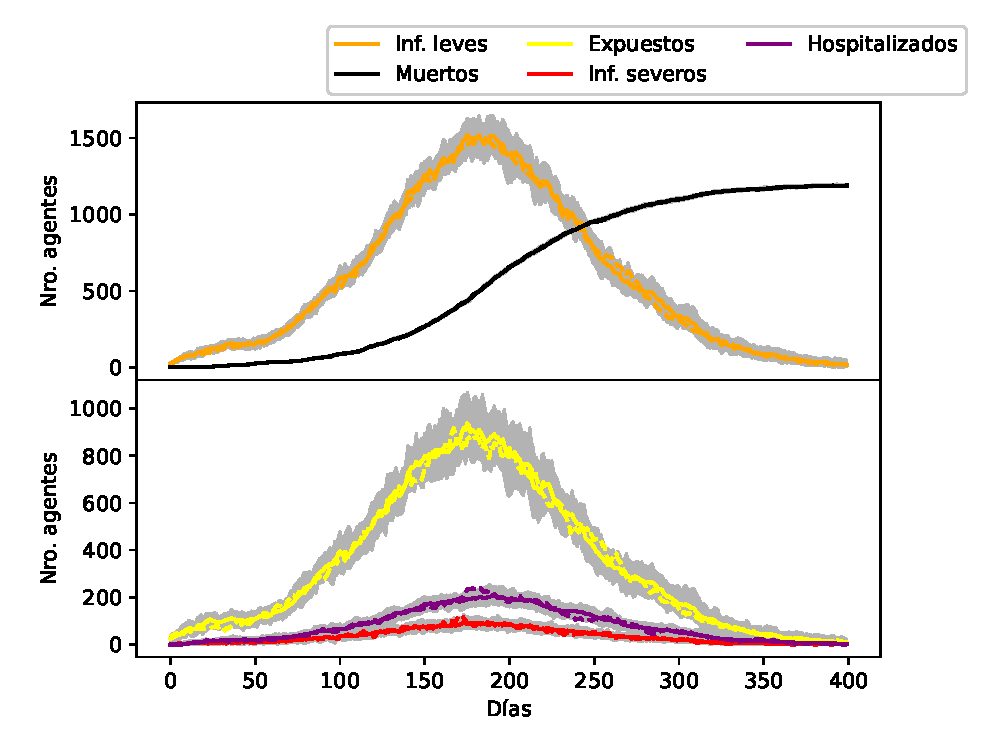
\includegraphics[width=0.75\textwidth]{abm_state_vars_moving_lambda.eps}
    \caption{Estimaciones de las variables de estado $I_M$ y $D$ en el panel superior y de $E$, $I_S$ y $H$ en el inferior. En líneas continuas las medias, en gris los miembros del ensamble y en líneas intermitentes los valores reales.}
    \label{fig:abm_state_vars_moving_lambda}
\end{figure}
\begin{figure}[h]
    \centering
    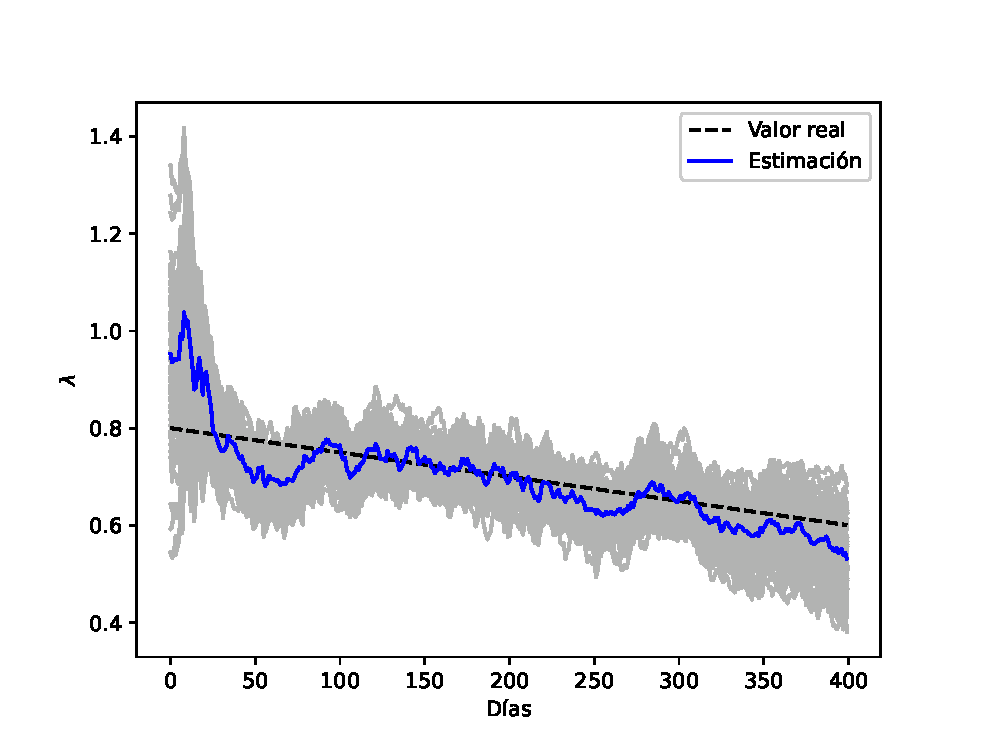
\includegraphics[width=0.75\textwidth]{abm_moving_lambda.eps}
    \caption{Estimaciones de $\lambda$. Media en azul y miembros del ensamble en gris. La línea intermitente indica el valor real.}
    \label{fig:abm_moving_lambda}
\end{figure}
\begin{figure}[h]
    \centering
    \includegraphics[width=0.75\textwidth]{abm_housing_dist_moving_lambda.eps}
    \caption{Proporción de infectados por tipo de hogar. Cada panel corresponde a distintos tamaños de hogar desde 1 habitante en panel superior a hogares de 5 habitantes en el panel inferior. Las líneas punteadas indican la proporción de habitantes en total (sin considerar estado epidemiológico) por cada tipo de hogar. Las líneas verdes señalan las proporciones de infectados de la corrida natural y las rojas las medias de las estimaciones mientras que las grises son las de los miembros de ensamble.}
    \label{fig:abm_housing_dist_moving_lambda}
\end{figure}

La estructura dada por la distribución de agentes en hogares no es informada de manera directa por las observaciones puesto que estas sólo están diferenciadas por barrio. El sistema sin embargo mantiene una población de agentes por cada miembro de ensamble y es posible evaluar cómo se distribuyen las infecciones en los distintos tipos de hogares. Nuestra parametrización del modelo considera casas con un mínimo de un solo habitante hasta un máximo de cinco. En cada día de asimilación computamos qué proporción de infectados corresponde a cada tamaño de hogar: los resultados se muestran en la Figura \ref{fig:abm_housing_dist_moving_lambda}. Cuando hay menos infecciones, es decir antes y después del pico epidémico las estimaciones tienen varianza más alta y son menos precisas mientras que durante el pico de infecciones la dispersión es mucho menor y las estimaciones más certeras. Podemos comparar la proporción de infectados en cada tipo de hogar con la proporción total de agentes residentes en cada tipo de hogar sin importar su estado epidemiológico. En casas más pequeñas la proporción estimada de infecciones es menor a la proporción de agentes que habitan en ese tipo de hogar. Lo opuesto sucede en casas de mayor tamaño. Esto se debe a que debido a los contactos domésticos la infección se dispersa con mayor rapidez en hogares con más habitantes. A su vez, la proporción de infectados en hogares más grandes es mayor al comienzo de la epidemia y menor hacia el final porque son los hogares que más rápidamente se saturan de inmunes (por infectarse más rápidamente).

\subsubsection{Seguimiento de la microescala}

Realizamos un experimento en el que evaluamos, en distintos niveles de agrupamiento, qué cantidad de agentes coinciden en su estado epidemiológico,  comparando entre las estimaciones y la corrida real. El objetivo del experimento es comparar la evolución del estado en la micro-escala entre la población real de agentes y las de los miembros del ensamble. Contaremos la cantidad de agentes que tienen el mismo estado epidemiológico pero considerando diferentes agrupamientos de agentes. Cada agente tiene un número de identificación (id); la primera métrica consistirá en comparar el estado epidemiológico de los agentes id por id. La segunda métrica consistirá en comparar casa por casa para chequear coincidencias utilizando el id que posee cada casa. Para la tercera métrica agruparemos los agentes de acuerdo al tamaño de hogar en el que habitan. La última métrica agrupa agentes de acuerdo al tamaño de hogar y el barrio en que habitan. La única métrica que distingue agentes por su id es la primera, para el resto contamos las coincidencias simplemente contando la cantidad de agentes en la misma categoría epidemiológica. Estas métricas permiten evaluar el estado microscópico del sistema y sus desviaciones respecto al estado real. Utilizamos $N_{loc} = 4$ barrios y en lugar de utilizar un valor de $\lambda$ global consideramos un valor distinto para cada locación, de manera que tenemos un vector de $N_{loc}$ componentes $\lambda = (1.0\;\; 0.8\;\; 0.9\;\; 0.7)$. 

La configuración inicial de los agentes para la corrida real y los miembros del ensamble es la misma por lo que al comienzo el porcentaje de coincidencias es 100\% para todas las métricas. Para evaluar el impacto de la asimilación  producimos además 100 simulaciones sin ningún tipo de asimilación para poder comparar los resultados. Estas serán diferentes a la trayectoria real debido a la estocasticidad del modelo.

La Figura \ref{fig:abm_matchings} muestra los resultados para ambos métodos de ajuste de los agentes y para las simulaciones sin asimilación de datos. Cada panel muestra una de las métricas. La metodología de redistribución aleatorizada y de cascada hacia atrás producen resultados similares en todos los casos. Las trayectorias de las métricas para las corridas independientes tienen una gran dispersión mientras que cuando se asimilan datos estas están contenidas. Para las métricas de id de agentes y de casas, que son las que evalúan a una escala más microscópica, se puede ver que el porcentaje de coincidencias cae, se recupera un poco y finalmente se estabiliza tanto para las corridas con EnKF como para las simulaciones independientes. Estas últimas son ligeramente más consistentes con la corrida real en la primera etapa en que todas las métricas caen. Esto es posiblemente debido a que la metodología de ajuste debe modificar el estado de agentes para lograr la consistencia con las variables macroscópicas mientras que las simulaciones independientes mantienen en mayor medida la estructura inicial de la población de agentes.
\begin{figure}[h]
    \centering
    \includegraphics[width=0.75\textwidth]{abm_matchings.pdf}
    \caption{Proporción de aciertos (cantidad de agentes con coincidencia en el estado epidemiológico respecto a la corrida natural) para las 4 métricas distintas (una en cada panel). Las líneas grises corresponden a las corridas independientes y las líneas negras son sus respectivas medias. Las líneas rojas y azules con transparencias corresponden a los miembros de ensamble para las corridas con EnKF para el método de resdistribución aleatorizada (azul) y de cascada hacia atrás (rojo)}
    \label{fig:abm_matchings}
\end{figure}

En la escala de tamaños de hogares el EnKF mantiene un porcentaje alto de coincidencias (mayor al 90\% para ambas metodologías de ajuste). En cambio, las simulaciones independientes muestran una gran variabilidad. El resultado para la métrica que agrupa por tipo de hogar y barrio da resultados similares. Algunas de las trayectorias de las simulaciones independientes tendrán picos epidémicos que no coinciden con el de la trayectoria real por lo que es esperable que las métricas para estas corridas decrezcan. El porcentaje de coincidencias luego se recupera puesto que el tamaño final de la epidemia será similar para la corrida real y las simulaciones y la mayor parte de los agentes estará en la categoría de susceptibles o recuperados. Por su parte, para el EnKF tenemos un buen nivel de coincidencias para estas métricas debido a que al asimilar datos, las trayectorias del ensamble pueden detectar el pico epidémico y sincronizar con el estado real en esta escala. Es importante notar que las observaciones en estos experimentos están separadas por barrio pero no son explícitamente informativas respecto a las infecciones en distintos tamaños de hogar. Aún así el porcentaje de coincidencias es bastante alto para estas métricas. La proporción de coincidencias considerando ids de agentes o agrupando por casas particulares es similar usando asimilación de datos o no haciéndolo. Esto es posiblemente porque los ids de agentes o de casas no juegan un rol particular en las dinámicas de contagio. En cambio, el tipo de hogar sí tiene un efecto en la dispersión de la enfermedad y por lo tanto este es capturado por el EnKF.

\subsubsection{Estimación de casos no detectados}

Es esperable que los datos de infecciones de COVID-19 reportados por los sistemas nacionales de salud estén afectados por el subreporte de casos ya que existen casos muy leves o incluso asintomáticos que no son contabilizados. Para evaluar si a través del sistema de asimilación podemos capturar los casos no reportados en las observaciones, modificamos levemente nuestro modelo y consideramos que las infecciones leves tienen una posibilidad $q_A$ de ser asintomáticos y por lo tanto no estar contabilizados en los datos observacionales. Para el experimento utilizamos una configuración similar a la de los experimentos anteriores pero tomando un valor fijo de $\lambda = 0.8$ e introduciendo $q_A$ en el estado aumentado. Para dar cuenta de los asintomáticos agregamos dos nuevas categorías epidemiológicas: los infectados asintomáticos $I_A$ y los recuperados de una infección asintomática $R_A$. El diagrama de las categorías epidemiológicas se puede representar entonces como en la Figura \ref{dia:abm_unobserved}. También sería posible simular un escenario similar considerando coeficientes desconocidos en el operador observacional $\v H_t$ que serían estimados mediante estado aumentado.

\begin{figure}[h]
    \captionsetup{width=0.5\textwidth}
    \begin{center}
        \tikzstyle{block} = [rectangle, draw, fill=blue!20, 
        text width=4em, text centered, rounded corners, minimum height=3em]
        \tikzset{line/.style={draw, very thick, color=black!100, -latex'}}
        \centering
        \begin{tikzpicture}[node distance = 2cm, auto]
            \tikzstyle{block} = [rectangle, draw, fill=blue!20, 
            text width=2em, text centered, rounded corners, minimum height=3em]
            
            % Place nodes
            \node [block] (S) {$S$};
            \node [block, right of=S] (E) {$E$};
            \node [block, above right = 0.75cm and 4cm of E] (IA) {$I_A$};
            \node [block, right = 4cm of E] (IM) {$I_M$};
            \node [block, below right = 0.75cm and 4cm of E] (IS) {$I_S$};
            \node [block, right of=IS] (H) {$H$};
            \node [block, right of=H] (D) {$D$};
            \node [block] (R) at (IM-|D) {$R$};
            \node [block] (RA) at (IA-|R) {$R_A$};

            % Draw edges
            \draw[line] (S) -- (E);
            \draw[line] (E) |- ++(2.5cm,1cm) |- node [above right = 0cm and 0.4cm, align=center] {$q_A$} (IA);
            \draw[line] (E) |- node [above right = 0cm and 0.8cm, align=center] {$1-q_S$} ++(2.5cm,1cm) |- node [above right = 0cm and 0.4cm, align=center] {$1-q_A$} (IM);
            \draw[line] (E) |- node [above right = 0cm and 0.8cm, align=center] {$q_S$} (IS);
            \draw [line] (IM) -- (R);
            \draw [line] (IA) -- (RA);
            \draw [line] (IS) -- (H);
            \draw [line] (H) -- (D);
            \draw [line] (H) -- node [left = 0.01cm] {$1-q_D$} (R);
            \draw [line] (H) -- node [below] {$q_D$} (D);
        \end{tikzpicture}
    \end{center}
    \caption{Diagrama para el epiABM con asintomáticos}
    \label{dia:abm_unobserved}
\end{figure}

Las variables observadas serán los confirmados acumulados como la suma de $I_M$, $I_S$, $R$ y $D$ y los muertos acumulados, $D$. Además incorporaremos una nueva variable observacional que llamaremos positividad global. Notemos que para los casos confirmados no incorporamos ni a $I_A$ ni a $R_A$ puesto que estos casos pasarían en principio inadvertidos para el sistema de reportes. La positividad global será el resultado de un testeo diario aleatorio a un porcentaje fijo de la población. Los tests darán positivos para $I_M$, $I_S$, $I_A$ y $H$ por lo que estas observaciones sí podrán capturar algo de información respecto a la cantidad de asintomáticos. Los tests son globales y no están separados por locación por lo que dan una idea de la circulación global del virus. El error observacional de esta variable no será Gaussiano aditivo sino que será el error de muestreo que resulta de la aleatoriedad de los tests. Asumimos que un 1\% de la población es testeada cada día. En la práctica los testeos no se suelen hacer completamente al azar sino que se hacen sobre casos posibles pero estos valores podrían ser utilizados para calcular aproximaciones de la positividad global. El valor de $q_A$ será estimado mediante estado aumentado y se espera que las correlaciones de la positividad global con este parámetro permitan su inferencia.

La Figura \ref{fig:abm_tests} muestra los resultados para los infectados leves, los asintomáticos y la positividad global y el testeo. El comportamiento de los asintomáticos es capturado por el EnKF pero como es de esperarse las estimaciones de los infectados leves son más precisas. Esto es porque los asintomáticos son solo informados a través de la positividad global mientras que los infectados leves también son observados mediante los infectados acumulados por barrio. La discrepancia entre los asintomáticos y el valor real de esta variable está correlacionada con la discrepancia entre la positividad global y estimada. Esto sugiere que mientras más sepamos sobre la circulación general del virus, mejor podrá ser la inferencia sobre los casos no reportados. La Figura \ref{fig:abm_tests_asymptomatic_prob} muestra las estimaciones de la probabilidad $q_A$. Se ve en los primeros ciclos de spin-up una reducción de la varianza inicial y luego el ensamble sincroniza con el valor real. Cuando la positividad es menor, antes y después del pico epidémico, la varianza del ensamble es mayor que durante el pico epidémico, en donde las estimaciones son más precisas y de menos varianza. Este efecto se debe a que la positividad sólo será informativa de la proporción de asintomáticos en la medida que haya suficientes casos como para que las correlaciones entre los testeos y el parámetro sean lo bastante fuertes.
\begin{figure}[h]
    \centering
    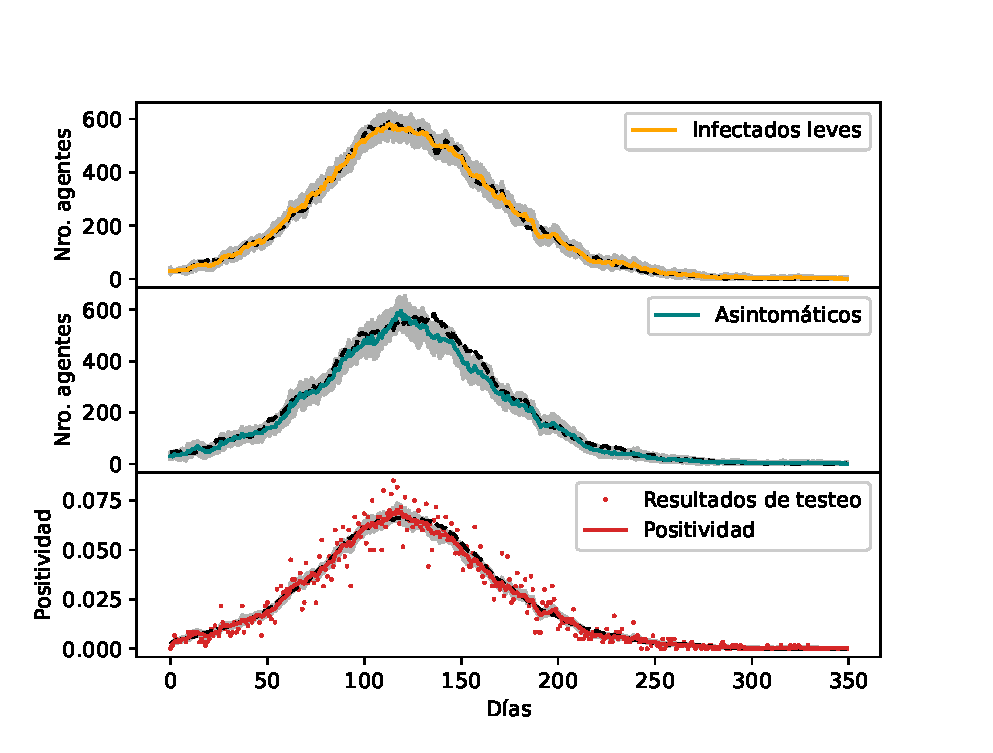
\includegraphics[width=0.75\textwidth]{abm_tests.eps}
    \caption{Estimaciones de infectados leves, asintomáticos y positividad global. Las líneas grises corresponden a los miembros del ensamble y las continuas a sus medias. Las líneas intermitentes indican los valores reales. En el panel inferior los puntos indican la positividad observada del testeo.}
    \label{fig:abm_tests}
\end{figure}
\begin{figure}[h]
    \centering
    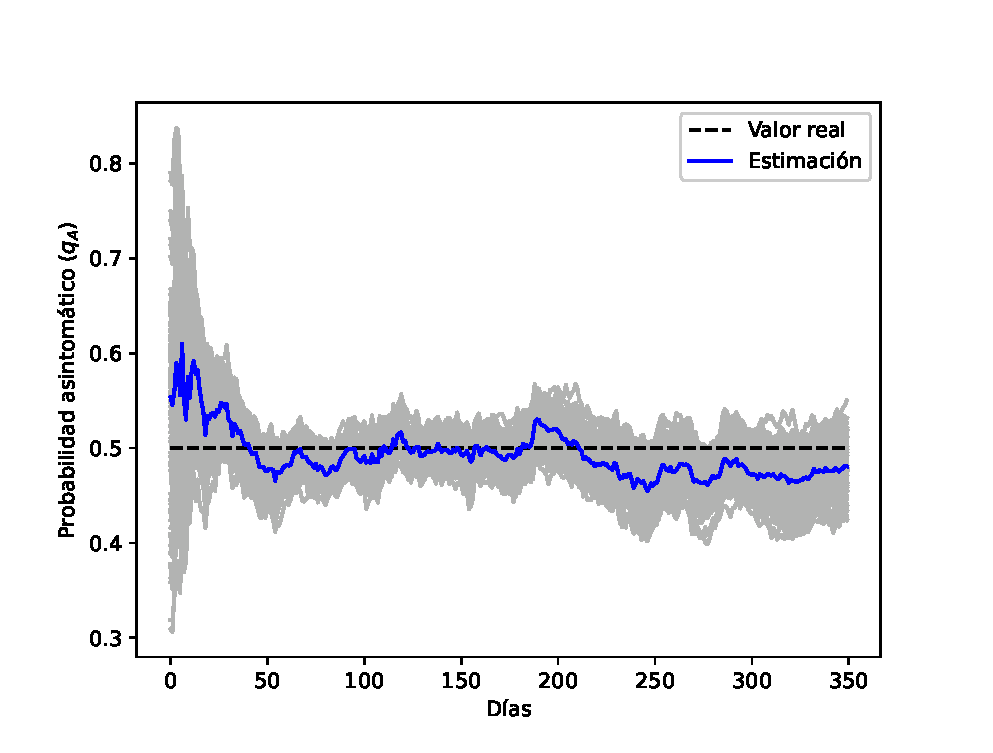
\includegraphics[width=0.75\textwidth]{abm_tests_asymptomatic_prob.eps}
    \caption{Estimaciones de la probabilidad $q_A$ de que un infectado leve sea asintomático. Las líneas grises indican a los miembros del ensamble, y la azul a su media. El valor real se representa con la línea intermitente}
    \label{fig:abm_tests_asymptomatic_prob}
\end{figure}

\subsubsection{Respuesta al error de modelo}

En este experimento buscamos evaluar si la metodología es lo suficientemente robusta como para responder en situaciones en que el modelo está erróneamente especificado. Para ello diseñamos el experimento de manera que la corrida natural y las del EnKF tienen configuraciones diferentes. Para generar las observaciones sintéticas, el número de contactos diarios va a ser muestreado, no de una Poisson como hicimos hasta ahora, sino de una distribución geométrica con parámetro $p = 0.5$. Por el otro lado, para la inferencia con EnKF usaremos la distribución de Poisson como en los experimentos anteriores. Adicionalmente usaremos distintas distribuciones de hogares: para la corrida natural tomaremos $p_H = (0.33\;\; 0.27\;\; 0.2\;\; 0.13\;\; 0.07)$ lo que resulta en que las casas con más agentes son más infrecuentes que las que tienen menos habitantes, lo cual es esperable en un medio urbano. Para el EnKF utilizaremos esta distribución pero también repetiremos el experimento con una distribución uniforme de hogares $p_H = (0.2\;\; 0.2\;\; 0.2\;\; 0.2\;\; 0.2)$ y otra ``desbalanceada'' $p_H = (0.07\;\; 0.13\;\; 0.2\;\; 0.27\;\; 0.33)$ en la que los hogares de más habitantes son más frecuentes que los de menos. La utilización de distribuciones de hogares diferentes va a resultar en distintas dinámicas de propagación debido a la variación en la estructura de la red de contactos. El parámetro $\lambda$ se estima mediante estado aumentado.

La Figura \ref{fig:abm_housing_dist_KL} muestra las trayectorias de las estimaciones de $\lambda$ para los distintos escenarios de distribución de hogares. La distribución para el número de contactos para el EnKF es una Poisson mientras que para la corrida real es geométrica, por lo tanto la estimación de $\lambda$ debería parametrizar al número de contactos diarios de manera que se parezca lo más posible a una geométrica. Para evaluar el parecido entre distribuciones entonces calculamos para una grilla de valores de $\lambda$ la divergencia de Kullback-Leibler (KL) entre la Poisson y la verdadera distribución geométrica. Esta cantidad codifica cuánta información se pierde al utilizar la distribución Poisson respecto a la geométrica. En la Figura \ref{fig:abm_housing_dist_KL} también se muestra la divergencia KL junto con las estimaciones de $\lambda$. Estas están en regiones de baja divergencia KL: esto significa que el sistema se auto-calibra buscando el valor de $\lambda$ que mejor pueda reproducir las características del modelo original. La mejor estimación en términos de divergencia KL es para la corrida que utiliza la distribución real de hogares, lo cual es esperable. La distribución uniforme de hogares tiene más casas de mayor tamaño y la desbalanceada aún más. Esto causa una dispersión más rápida de la enfermedad debido a que habrá más contactos domésticos. El hecho de que las estimaciones de $\lambda$ sean menores en estos casos se debe a que el sistema se auto-calibra y por lo tanto compensa por la distribución de hogares incorrecta que produce un mayor número de contactos domésticos (los cuales tienen mayor probabilidad de ser contagiosos).
\begin{figure}[h]
    \centering
    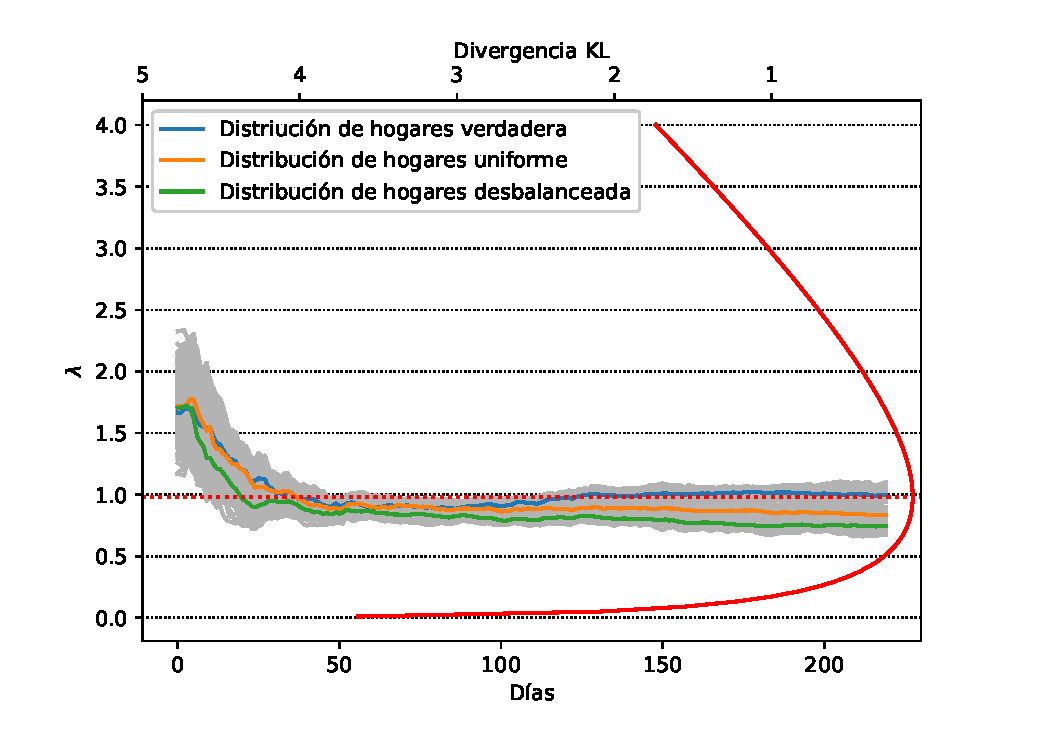
\includegraphics[width=0.75\textwidth]{abm_housing_dist_KL.eps}
    \caption{Estimaciones de $\lambda$ para tres escenarios de distribución de hogares distintas. La curva roja representa a la divergencia KL y sus valores están en el eje superior del gráfico. Las líneas grises representan a miembros del ensamble y las líneas sólidas correspondientes a sus medias}
    \label{fig:abm_housing_dist_KL}
\end{figure}

\subsection{Datos CABA, Argentina}

Para evaluar el sistema con datos realistas realizamos un experimento con los datos de COVID-19 de CABA, Argentina, provistos por el Ministerio de Salud y publicados con actualizaciones diarias en \url{https://data.buenosaires.gob.ar}. La distribución de hogares y la población es tomada de datos censales disponibles en el mismo sitio. CABA se divide en 15 comunas. Tomaremos a cada una de ellas como un barrio para el modelo (a pesar de que cada comuna puede estar compuesta por más de un barrio). Los datos están agrupados de acuerdo a las distintas comunas. Utilizaremos como observaciones sobre el sistema a los infectados acumulados y las muertes acumuladas. Consideraremos que el parámetro $\lambda$ es el mismo para todas las comunas y lo estimaremos mediante estado aumentado. Para la matriz de contacto consideraremos que la mitad de los contactos casuales son dentro de la misma comuna y la otra mitad están distribuidos de manera proporcional a la densidad poblacional de las otras comunas. Utilizamos $N_a = 3 \cdot 10^5$ agentes pero la población de CABA es aproximadamente $3 \cdot 10^6$ por lo que escalamos hacia abajo los datos en 10.

La Figura \ref{fig:abm_caba_data_lambda} muestra las estimaciones de $\lambda$. Como este parámetro codifica el número de contactos que un agente tiene por día es esperable que esté correlacionado con el número de infecciones confirmadas diarias y de hecho se puede ver que tienen una tendencia similar. Esto sucede porque las probabilidades de infección, $\beta_C$ y $\beta_D$, se consideran constantes durante la simulación por lo que los cambios en las infecciones diarias van a ser explicados por cambios en $\lambda$ con el correspondiente desfasaje debido al tiempo de incubación. La evolución de la tasa de contactos estimada es consistente con los tres picos epidémicos en Argentina hasta mediados de 2021.
\begin{figure}[h]
    \centering
    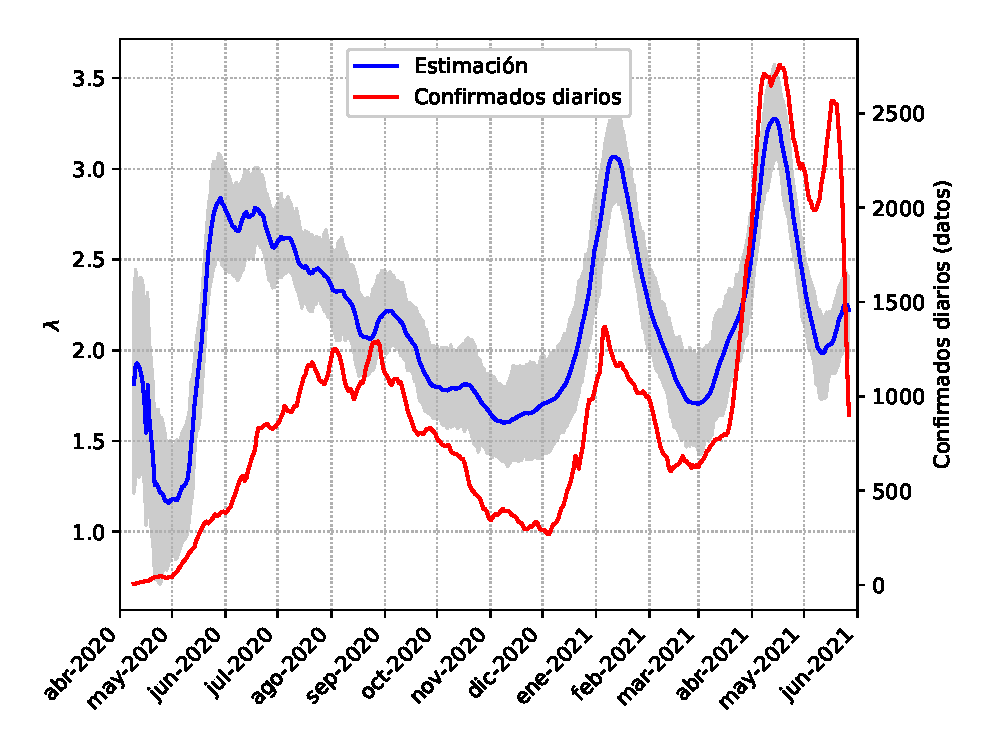
\includegraphics[width=0.75\textwidth]{abm_caba_data_lambda.eps}
    \caption{Estimaciones de $\lambda$ junto a los casos diarios confirmados suavizados mediante una media móvil de 7 días (estos valores se representan en el eje derecho de la gráfica). Los miembros del ensamble se indican con líneas grises.}
    \label{fig:abm_caba_data_lambda}
\end{figure}

Es importante notar que sólo estimamos el parámetro $\lambda$ dejando al resto fijo, cuando en realidad existen múltiples efectos que pueden influir en la propagación de la enfermedad. Esto significa que el ajuste del modelo a los datos se da a través de $\lambda$ a pesar de que puede haber sido otro fenómeno el que provocó un determinado cambio en la tendencia de los datos. Por ejemplo, una disminución de los casos causada por el mayor uso de tapabocas debería ser representado mediante una baja en la probabilidad de infecciones casuales $\beta_C$ pero, dado que este parámetro está fijo, el cambio será capturado por $\lambda$. A pesar de que esto puede ser impreciso, notamos que intentar estimar muchos parámetros con efectos similares en los datos pude llevar a una sobreparametrización y falta de identificabilidad.
\begin{figure}[h]
    \centering
    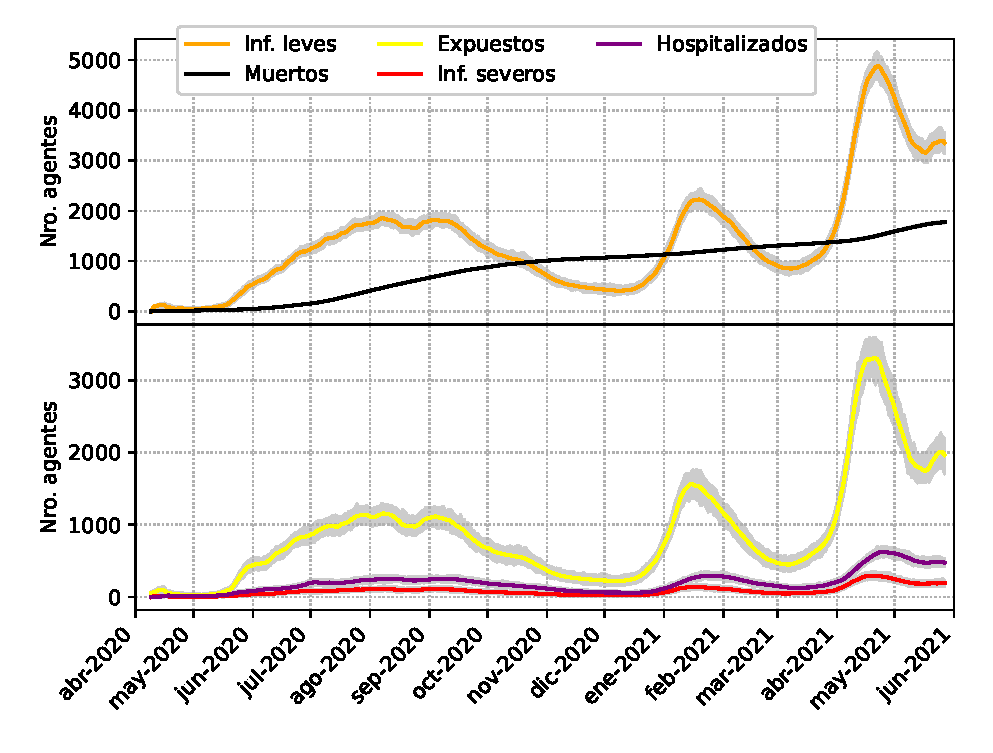
\includegraphics[width=0.75\textwidth]{abm_caba_data_state_vars.eps}
    \caption{Estimaciones de las variables de estado $I_M$ y $D$ en el panel superior y de $E$, $I_S$ y $H$ en el inferior. En líneas continuas las medias, en gris los miembros del ensamble.}
    \label{fig:abm_caba_data_state_vars}
\end{figure}

La Figura \ref{fig:abm_caba_data_state_vars} muestra algunas de las variables agregadas del sistema sumadas a través de todos los barrios. Las muertes acumuladas tienen menor varianza que el resto de las variables. De manera similar a los experimentos con observaciones sintéticas, esto se debe a que las muertes son directamente observadas mientras que las otras variables son observadas a través de la suma de varios estados epidemiológicos.
\begin{figure}[h]
    \centering
    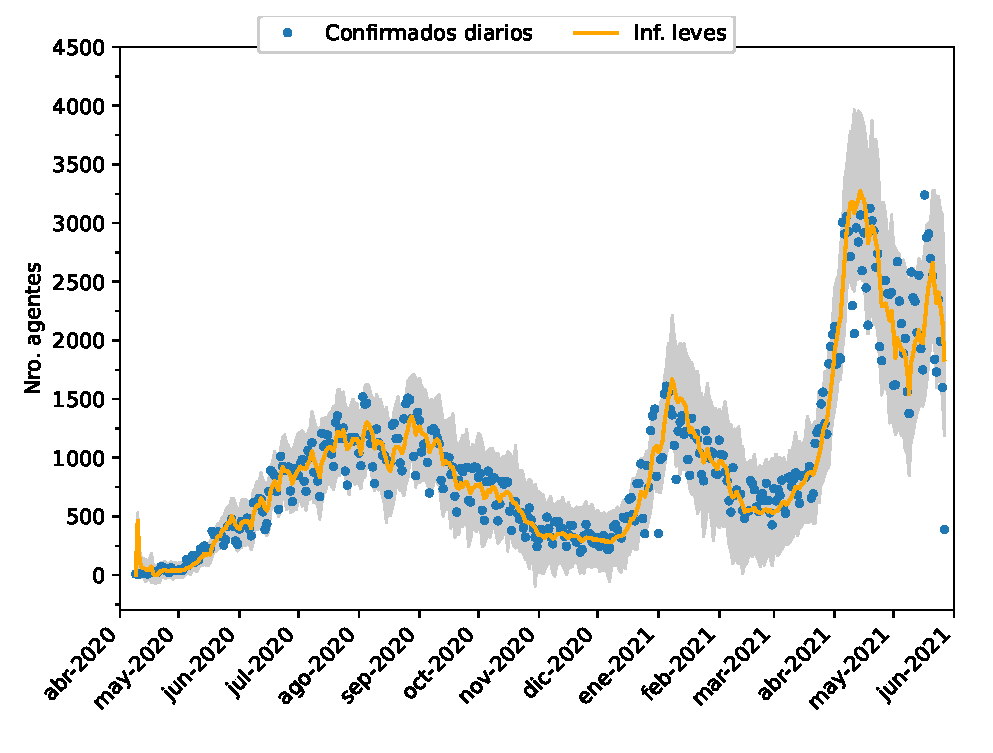
\includegraphics[width=0.75\textwidth]{abm_caba_data_aggregated.eps}
    \caption{Estimaciones de infectados diarios en toda la ciudad. Las líneas grises indican miembros del ensamble y la línea sólida su media. Las observaciones se representan con puntos.}
    \label{fig:abm_caba_data_aggregated}
\end{figure}

En la Figura \ref{fig:abm_caba_data_aggregated} se puede ver el número de casos diarios. En los datos se puede ver el efecto del subreporte de los fines de semana pero las estimaciones suavizan en parte este efecto. La estimación entonces es más cercana a lo que esperamos que es el estado verdadero. La Figura \ref{fig:abm_caba_data_disaggregated} se muestran los mismos valores pero desagregados por comuna. Todas ellas tienen tendencias similares con algunas diferencias en la forma de los picos epidémicos pero estos efectos son capturados por el EnKF.

\begin{figure}[h]
    \centering
    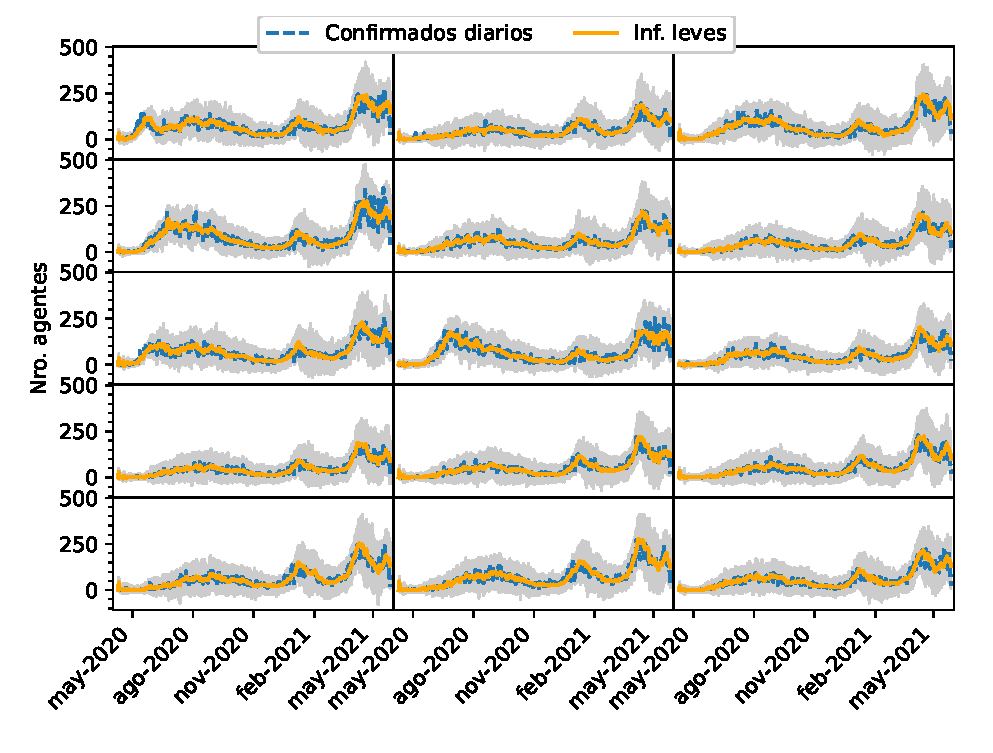
\includegraphics[width=0.75\textwidth]{abm_caba_data_disaggregated.eps}
    \caption{Estimaciones de infectados diarios en cada comuna de la ciudad. Las comunas están numeradas del 1 al 15 y están ordenadas en la gráfica de izquierda a derecha y de arriba a abajo. Las líneas grises indican miembros del ensamble y la línea sólida su media. Las observaciones se representan con líneas intermitentes.}
    \label{fig:abm_caba_data_disaggregated}
\end{figure}

\subsection{Discusión}

En nuestro modelo epidemiológico, la evaluación experimental de las metodologías que propusimos para aplicar asimilación de datos por ensambles en ABMs da muestras prometedoras para la inferencia en este tipo de sistemas. Las metodologías de ajuste de agentes descriptas en la Sección \ref{sec:agents_adjustment} dan resultados similares y pueden recuperar los valores reales de las variables macroscópicas. En principio, las estimaciones sobre el estado microscópico de los agentes depende de la granularidad de las observaciones y de cuánto informen estas sobre la microescala. Por otro lado, los experimentos muestran que se puede sacar provecho del método de estado aumentado para la estimación de parámetros del modelo incluso en situaciones de especificaciones incorrectas de modelo como se muestra en los resultados de la Figura \ref{fig:abm_housing_dist_KL}. En cuanto a su aplicación con datos reales, la correlación entre la incidencia diaria de casos y el parámetro $\lambda$ que se puede ver en la Figura \ref{fig:abm_caba_data_lambda} sugiere que el sistema responde a los cambios del escenario epidemiológico que subyace en los datos. Es importante notar que en general, tanto en ABMs como en modelos de ecuaciones diferenciales, cuando se utilizan parámetros con efectos similares sobre las trayectorias observadas del sistema los efectos pueden no ser diferenciados por la técnica de asimilación. Esto incentiva la utilización de modelos parsimoniosos para poder sacar provecho de las herramientas de inferencia que aporta la asimilación de datos.
